\documentclass[border=5pt]{standalone}
\usepackage{tikz}
\usetikzlibrary{arrows.meta, 3d, perspective, calc}
\usepackage{amsmath}
\begin{document}
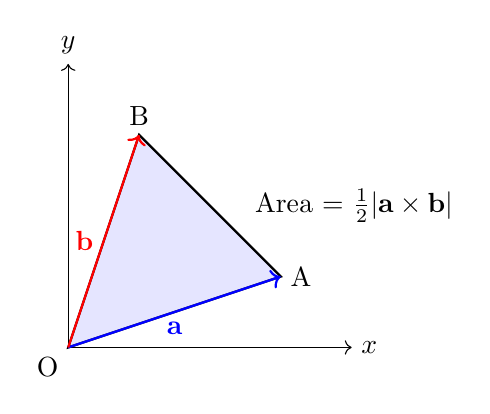
\begin{tikzpicture}[scale=0.9]
    % Coordinate axes
    \draw[->] (0,0) -- (4,0) node[right] {$x$};
    \draw[->] (0,0) -- (0,4) node[above] {$y$};

    % Triangle
    \draw[thick, fill=blue!10] (0,0) -- (3,1) -- (1,3) -- cycle;

    % Position vectors
    \draw[->,thick,blue] (0,0) -- (3,1) node[midway,below] {$\mathbf{a}$};
    \draw[->,thick,red] (0,0) -- (1,3) node[midway,left] {$\mathbf{b}$};

    % Labels
    \node at (0,0) [below left] {O};
    \node at (3,1) [right] {A};
    \node at (1,3) [above] {B};

    % Area formula
    \node[right] at (2.5,2) {Area = $\frac{1}{2}|\mathbf{a} \times \mathbf{b}|$};
\end{tikzpicture}
\end{document}
